\chapter{Preparing for Hadoop Installation}\label{chap:2}
In this chapter, we will cover:
\begin{itemize}
  \item Choosing hardware for cluster nodes
  \item Designing the cluster network
  \item Configuring the cluster administrator machine
  \item Creating kickstart file and boot media
  \item Installing the Linux operating system
  \item Installing Java and other tools
  \item Configuring SSH
\end{itemize}
\section{Introduction}
The configuration of a Hadoop cluster is a systematic project, especially, due to its large scale and the distributed property. Efforts are needed in choosing the proper storage and computing hardware, designing the interconnected network and installing and configuring the operating system and so on.

In a Hadoop cluster, different types of nodes may require different hardware configurations. For example, the JobTracker on a master node schedules jobs and assigns tasks to proper slave nodes for execution and the NameNode on the master node manages the metadata for files and data blocks. In addition, the master node is a critical failure point in a default cluster configuration, which configures only one master node. A critical requirement for the master node is to be responsive and reliable. On the other hand, a slave node is responsible for hosting data blocks and running tasks upon the data blocks. Because of the built-in cluster level failure resilience, the reliability requirement for a slave node is not as strict as a master node. But a slave node should have enough storage space and computing power to satisfy the storage and computing requirements.

Similarly, different Hadoop cluster sizes may have different configuration requirements. For example, for a small to medium sized cluster with up to a hundred slave nodes, the NameNode, JobTracker and SecondaryNameNode daemons can be put on the same master machine. When the cluster size grows up to hundreds even thousands of slave nodes, it becomes advisable to put these daemons on different machines. In this book, we assume to build a cluster with 5 slave nodes, which makes it reasonable to put the NameNode, JobTracker and SecondaryNameNode daemons on the same physical machine.

Nodes in a Hadoop cluster are interconnected through network devices such as switches and routers. Data will be transferred from one node to another over the network during different phases of a MapReduce job. There are many factors that can affect the performance of a Hadoop cluster, some of which have greater influence than others. For example, network segmentation caused by device failures can greatly degrade the cluster performance, while network speed and latency have much smaller influence comparatively. So, highly available and resilient network architecture is crucial for a Hadoop cluster.

Hadoop runs on Linux (although Windows operating systems are supported, it is still not stable at the time of writing this book). We need to install and configure Linux on all cluster nodes before the Hadoop installation process. If you have experience working with Linux, you may know that installing Linux on a single machine is straightforward by following the installation instructions. For example, we can burn the downloaded operating system ISO image onto a DVD optical disk and then boot and install the operating system using this DVD. However, the simple and straightforward installation method is too inefficient to be practical for a Hadoop cluster with a large number of nodes. We are going to explore more practical and efficient installation methods in this chapter.

Some operating system configuration is needed after installing the Linux operating system. For example, we need to configure users and groups, system security such as firewalls and SELinux. We also need to install the required Hadoop dependency software, Java and some optional tools that can improve cluster management efficiency.
\section{Choosing hardware for cluster nodes}
A Hadoop cluster contains two types of nodes: master node\index{master node} and slave node\index{slave node}. By default, the NameNode, SecondaryNameNode and JobTracker daemons reside on a master node; DataNode and TaskTracker daemons reside on slave nodes. Properly selecting hardware for these computing and storage nodes can maximize the efficiency of a Hadoop cluster. In this recipe, we will list suggestions on hardware selection for a computing node.
\subsection*{How to do it}
Although special requirements exist for a master node and a slave node, there is no gold standard for choosing optimal hardware for both types of nodes. It is reasonable to say that the hardware configuration is closely related to the properties of Big Data to be processed. In addition, the choice of hardware is an empirical and adaptive process with the changing requirements on a Hadoop cluster. For example, if the requirements for the throughput of a Hadoop cluster are high, we might need to choose high end CPUs and hard drives. If we have a large number of potential Hadoop users, we may need to upgrade the hardware configuration for both the master node and the slave nodes.

Empirically, we recommend the following configurations for a small to medium sized Hadoop cluster:

\begin{table}[h]
  \centering
  \begin{tabular}{lll}
    \toprule
    \textbf{Node Type} & \textbf{Node Components} & \textbf{Recommended Specification} \\ \midrule
    Master Node & CPU	& $\ge$ 2 Quad Core, 2.0GHz \\
    & RAM (Main Memory) & $\ge$ 16GB \\
    & Hard Drive & $\ge$ 2 x 1TB SATA II 7200 RPM HDD or SSD\footnote{HDD stands for Hard Disk Drive and SSD stands for Solid State Drive} \\
    & Network Card & $\ge$ 1Gbps Ethernet \\ \midrule
    Slave Node & CPU & $\ge$ 2 Quad Core \\
    & RAM (Main Memory) & $\ge$ 16GB \\
    & Hard Drive & $\ge$ 4 x 1TB HDD \\
    & Network Card & $\ge$ 1Gbps Ethernet \\ \bottomrule
  \end{tabular}
  \caption{Hadoop cluster hardware configuration recommendations}\label{tbl:cluster.hardware}
\end{table}
\subsection*{How it works}
On a Hadoop master node, the NameNode keeps the metadata such as permissions of each file in main memory. The amount of memory needed by a master node depends on the number of file system objects (for example, numbers of files and block replicas) to be created and tracked. The memory requirement will be high when the cluster is large. The SecondaryNameNode keeps a backup for the latest filesystem checkpoint mirrored from the NameNode, so its memory requirement is similar as the NameNode.

In default configuration, the master node is a single failure point. Higher end computing hardware and secondary power supplies are suggested.

In Hadoop, each slave node simultaneously executes a number of map or reduce tasks. The maximum number of parallel map/reduce tasks are known as map/reduce slots\index{slots}, which are configurable by a Hadoop administrator\index{Hadoop administrator}. Each slot is a computing unit consisting of CPU\index{CPU}, memory\index{memory} and disk I/O\index{disk I/O} resources. When a slave node was assigned a task by the JobTracker\index{JobTracker}, its TaskTracker\index{TaskTracker} will fork a JVM for that task, allocating a preconfigured amount of computing resources. In addition, each forked JVM also will incur a certain amount of memory requirements. Empirically, a Hadoop job can consume 1-2 GB memory for each CPU core. Higher data throughput requirement can incur higher I/O operations for the majority of Hadoop jobs. That's why higher end and parallel hard drives can help boost the cluster performance. To maximize parallelism, it is advisable to assign two slots for each CPU core. For example, if our slave node has two quad-core CPUs, we can assign $2 \times 4 \times 2 = 16$ (map only, reduce only or both) slots in total for this node.

In the simple equation, the first 2 stands for the number of CPUs of the slave node, the number 4 represents the number of cores per CPU and the second 2 means the number of slots per CPU core\index{CPU core}.
\subsection*{See also}
\begin{itemize}
  \item Designing the cluster network
  \item Managing HDFS cluster in Chapter \ref{chap:4}, Managing a Hadoop cluster.
  \item Chapter \ref{chap:7}, Tuning Hadoop cluster for best performance.
\end{itemize}

\section{Designing the cluster network}
Network\index{Network} is the backbone of a Hadoop cluster. Its stability is critical for the performance of the cluster. In this recipe, we will outline a few general rules for designing a Hadoop cluster network.
\subsection*{How to do it}
The network architecture for a small to medium sized cluster can be as simple as connecting the cluster nodes with one or more switches. Connection redundancy can add reliability to the network.
\begin{warning}
Warning! \\
Computing nodes in a Hadoop cluster should be configured within the same network segment (Local Area Network or LAN). Advanced features such as VLANs that can cause overhead are not recommended. And connecting nodes with a router is not recommended.
\end{warning}
The network architecture\index{network architecture} for Hadoop clusters with hundreds or thousands of nodes is much more complex. In a large cluster, the physical nodes are usually so small, for example blade server, that they can be mounted on racks. Each rack has a local switch that interconnects nodes on the save rack. These racks are then interconnected with more advanced switches.

Nodes on the same rack can be interconnected with 1Gbps (Gigabit per second) Ethernet switch. Cluster level switches then connect the rack switches with faster links such as 10Gbps optical fiber links and other networks like InfiniBand. The cluster-level switches may also interconnect with other cluster-level switches or even uplink to another higher level of switching infrastructure. With the increasing size of a cluster, the network, at the same time, will become larger and more complex. Connection redundancies for network high availability can also increase its complexity. In this book, we assume to discuss the basic network architecture design method. If you want to learn more advanced network design techniques, please refer to related books and online materials.

In general, the network architecture of medium sized cluster can be described with the following figure:
\begin{figure}[ht]
  \centering
  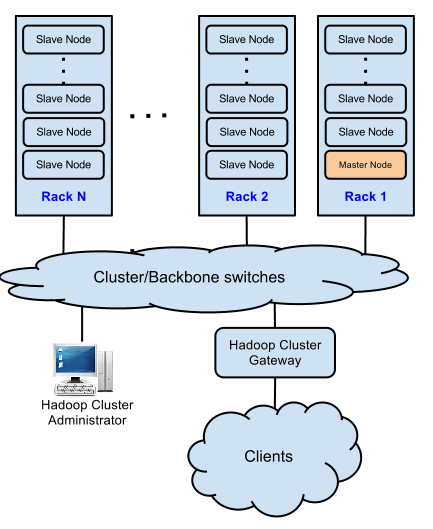
\includegraphics[width=.6\textwidth]{figs/5163os_02_01.png}
  \caption{Network Architecture of Hadoop Cluster}\label{fig:network.architecture}
\end{figure} 
In this figure, we assume there is a Hadoop cluster administrator machine and the clients connect to the cluster through a gateway\index{gateway}, through which Hadoop jobs can be submitted.
\subsection*{How it works}
The increasing bandwidth of network devices makes it possible for Hadoop to load and replicate large data sets across interconnected nodes. Resilient and scalable network architecture can secure the high data throughput and performance requirements for a Hadoop cluster.

\section{Configuring the cluster administrator machine}
As we have mentioned previously, the most efficient way to install Linux on a large number of machines is to install over the network. In this book, we assume to use the administrator machine as the installation server. We will learn steps to configure this server, including the configuration of the following two services: DHCP\index{DHCP} and FTP\index{FTP}.

\subsection*{Getting ready}
Before getting started, we assume that the cluster administrator machine has a 64bit Red Hat compatible Linux operating system installed. The hostname of the machine is hadoop.admin and an administrative user hdadmin has been created. This user should have \emph{sudo} privileges to install software packages, configure system services and so on. We also assume administrative tools such as a command line text editor has been installed on this machine. We will use these tools and commands directly in the upcoming recipes.

In this book, we assume to use CentOS\index{CentOS} 6.3 (which corresponds to Red Hat Enterprise Linux (RHEL) 6.3) as the Linux distribution. We will follow the Red Hat syntax for all the administrative commands, if you are using a Linux distribution other than CentOS, such as Debian, please refer to corresponding documentation.

Login to the administrator machine as hdadmin and change the hostname of the machine with command:
\lstset{style=bashstyle}
\begin{lstlisting}[language=bash]
$ sudo sed -i 's/\^HOSTNAME.*\$/HOSTNAME=hadoop.admin/' /etc/sysconfig/network
\end{lstlisting}
Create directories with command: \\
\verb|$ mkdir -v ~/mnt ~/isoimages ~/repo|

We will use directory ~/mnt as the mount point for ISO images. Directory \verb|~/isoimages| will be used to contain the original image files and directory ~/repo will be used as the repository folder for network installation.

Install DHCP and FTP servers on the machine with commands: 
\lstset{style=bashstyle}
\begin{lstlisting}[language=bash]
$ sudo yum -y install dhcp
$ sudo yum -y install vsftpd
\end{lstlisting}

We will use the DHCP server to assign IP addresses and bootstrap the operating system in the installation process and use the FTP server to host the installation packages.
\subsection*{Download the latest ISO image from a mirror}
The CentOS official site provides a worldwide mirrors list, including North America, European Countries, South America, Asia, Oceania, Middle East, Africa and other regions.

After selecting the nearest mirror, we can use either HTTP or FTP to download the image. Let's choose FTP as the download method by clicking the link in the corresponding line of the selected mirror. Then choose \verb|6.3/, isos/, x86_64/| consecutively. In this directory as shown in the following screenshot, we choose to download two ISO image\index{ISO image} files. Image file \verb|CentOS-6.3-x86_64-minimal.iso| contains all the necessary installation packages. And image file \verb|CentOS-6.3-x86_64-netinstall.iso| contains PXE network booting\index{PXE network booting} files used for booting over the network.
\begin{figure}[ht]
  \centering
  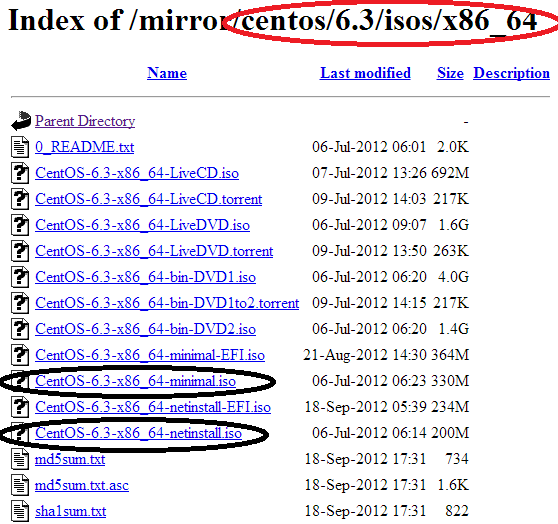
\includegraphics[width=.6\textwidth]{figs/5163os_02_02.png}
  \caption{Directory Listing of CentOS mirror site}\label{fig:centos.mirror}
\end{figure} 
If you are not sure about the architecture of the cluster machines, please refer to the product hardware menu.

Alternatively, we can use the following rsync to download the image:
\lstset{style=bashstyle}
\begin{lstlisting}[language=bash]
$ rsync rsync://mirror.its.dal.ca/centos/6.3/isos/x86_64/ CentOS-6.3-x86_64-netinstall.iso ~/isoimages
\end{lstlisting}

We can also use the following wget command to download the image file: 
\lstset{style=bashstyle}
\begin{lstlisting}[language=bash]
$ wget http://mirror.its.dal.ca/centos/6.3/isos/x86_64/ CentOS-6.3-x86_64-netinstall.iso -P ~/isoimages
\end{lstlisting}

Mount the image file with command:
\lstset{style=bashstyle}
\begin{lstlisting}[language=bash]
$ sudo mount $~/isoimages/ CentOS-6.3-x86_64-minimal.iso \
~/$mnt
\end{lstlisting}

Copy all the files to the \verb|~/repo| directory for FTP hosting with command: \\
\verb|$ cp -r $~/mnt/* ~/$repo|

Un-mount the ISO image with command: \\
\verb|$ sudo umount $~/$mnt|

The directory tree of the minimal image is similar to the following:
\begin{verbatim}
Insert the output of the directory listing.
\end{verbatim}

The directory tree of the netinstall image is similar to the following:
\begin{verbatim}
output of the directory listings.
\end{verbatim}
We can see from the directory trees that the minimal installation image file contains packages and boot images for system installation. The netinstall package only contains files for booting, including network booting files in the \verb|images/pxeboot| directory.

\subsection*{How to do it}
Use the following recipe configure DHCP server:

Use your favorite text editor to open file \verb|/etc/dhcp/dhcpd.conf| and change the following content:
\lstset{style=bashstyle}
\begin{lstlisting}
# Domain name
option domain-name "hadoop.cluster";

# DNS hostname or IP address
option domain-name-servers
dlp.server.world;

# Default lease time
default-lease-time 600;

# Maximum lease time
max-lease-time 7200;

# Declare the DHCP server to be valid.
authoritative;

# Network address and subnet mask
subnet 10.0.0.0 netmask 255.255.255.0 {

# Range of lease IP address, should be based
# on the size of the network
range dynamic-bootp 10.0.0.200 10.0.0.254;

# Broadcast address
option broadcast-address 10.0.0.255;

# Default gateway
option routers 10.0.0.1;
}
\end{lstlisting}

Start DHCP server with command: \\
\verb|$ sudo service dhcpd start|

The DHCP server start with the following message: \\
\verb|Starting dhcpd: [  OK  ]|

Make the DHCP server to survive a system reboot: \\
\verb|$ sudo chkconfig dhcpd --level 3 on|

Use the following recipe to configure FTP server: \\

Open file \verb|/etc/vsftpd/vsftpd.conf| with your favorite text editor and change the content according to the following list:
\lstset{style=bashstyle}
\begin{lstlisting}
# The FTP server will run in stand alone mode.
listen=YES

# Use Anonymous user.
anonymous_enable=YES

# Disable change root for local users.
chroot_local_user=NO

# Disable uploading and changing files.
write_enable=NO

# Enable logging of uploads and downloads.
xferlog_enable=YES

# Enable port 20 data transfer.
connect_from_port_20=YES

# Specify directory for hosting the Linux installation packages.
anon_ropot=~/repo
\end{lstlisting}

Start the FTP server with command: \\
\verb|$ sudo service vsftpd start|

The server will start with the following message: \\
\verb|Starting vsftpd: [  OK  ]|

Verify the FTP configuration with command: \\
ftp hadoop.admin

The configuration is successful if we get the following message:
\lstset{style=bashstyle}
\begin{lstlisting}
Trying 10.0.0.1...
Connected to hadoop.admin (10.0.0.1).
220 (vsFTPd 3.0.0)
Name (knoesis157:hdadmin):
\end{lstlisting}

\subsection*{See also}
\begin{itemize}
  \item Creating kickstart file\index{kickstart file} and boot media in Chapter 2, Preparing for Hadoop Installation.
  \item Installing the Linux operating system in Chapter 2, Preparing for Hadoop installation.
\end{itemize}

\section{Creating kickstart file and boot media}
Installing Linux on a large number of nodes with a kickstart file has a few advantages. For example, the installation process can be automated by specifying a list of to-be-installed packages and configuring system settings for the post installation process.

In this section, we will cover steps of creating a kickstart file and a USB boot media with the operating system image.
\subsection*{Getting ready}
A kickstart file is plain text file used for the automatic installation of Linux.

Prepare a USB flash drive with storage capacity larger than 512MB. The drive should have a single vfat file system partition. We can use the following command to check the filesystem type: \\
\verb|$ blkid|

We should see message similar to:
\lstset{style=bashstyle}
\begin{lstlisting}
/dev/sdb1 SEC_TYPE="msdos" LABEL="LIVE" UUID="07D9-051C" TYPE="vfat"
\end{lstlisting}

If the TYPE attribute is other than 'vfat\index{vfat}', use the following command to clear the first few blocks of the drive: \\
\verb|$ dd if=/dev/zero of=/dev/sdb1 bs=1M count=100|

Login to the administrative machine with command: \\
\verb|$ ssh hdadmin@hadoop.admin|

\subsection*{How to do it}
Use the following steps to create a kickstart file:

Install kickstart with command: \\
\verb|$ sudo yum install system-config-kickstart|

Use your favourite text editor to create a file \verb|ks.cfg| with the following content:
\lstset{style=bashstyle}
\begin{lstlisting}[language=bash]
#!/bin/bash
# Kickstart for CentOS 6.3 for Hadoop cluster.

# Install system on the machine.
install

# Use ftp as the package repository
url --url ftp://hadoop.admin/repo

# Use the text installation interface.
text

# Use UTF-8 encoded USA English as the language.
lang en_US.UTF-8

# Configure time zone.
timezone America/New_York

# Use USA keyboard.
keyboard us

# Set bootloader location.
bootloader --location=mbr --driveorder=sda rhgb quiet

# Set root password
rootpw  --password=hadoop

################################
# Partion the hard disk
################################

# Clear the master boot record on the hard drive.
zerombr yes

# Clear existing partitions.
clearpart --all --initlabel

# Create /boot partition, size is in MB.
part /boot --fstype ext3 --size 128

# Create / (root) partition.
part / --fstype ext3 --size 4096 --grow --maxsize 8192

# Create /var partition.
part /var --fstype ext3 --size 4096 --grow --maxsize 8192

# Create Hadoop data storage directory.
part /hadoop --fstype ext3 --grow

# Create swap partition, 16GB, double size of the main memory.
# Change size according to your hardware memory configuration.
part swap --size 16384

#################################
# Configure Network device.
#################################

# Use DHCP and disable IPv6.
network --onboot yes --device eth0 --bootproto dhcp --noipv6

# Disable firewall.
firewall --disabled

# Configure authorization.
authconfig --enableshadow

# Put Selinux in permissive mode.
selinux --permissive

############################################
# Specify packages to install.
############################################

# Automatically resolve package dependencies,
# exclude installation of documents and ignore missing packages.
%packages --resolvedeps --excludedocs --ignoremissing

# Install core packages.
@Base

# Don't install OpenJDK.
-java

# Install wget.
wget

# Install the vim text editor.
vim

# Install the Emacs text editor.
emacs

# Install rsync.
rsync

# install nmap network mapper.
nmap

%end

####################################
# Post installation configuration.
####################################

# Enable post process logging.
%post --log=~/install-post.log

# Create Hadoop user hduser with password hduser.
useradd -m -p hduser hduser

# Create group Hadoop.
groupadd hadoop

# Change user hduser's current group to hadoop.
usermod -g hadoop hduser

# Tell the nodes hostname and ip address of the admin machine.
echo "10.0.0.1 hadoop.admin" >> /etc/hosts

# Configure administrative privilege to hadoop group.

# Configure the kernel settings.
ulimit -u

#########################
# Startup services.
#########################

service sshd start
chkconfig sshd on

%end

# Reboot after installation.
reboot

# Disable first boot configuration.
firstboot --disable
\end{lstlisting}

Put the kickstart file into the root directory of the FTP server with command: \\
\verb|$ cp ks.cfg ~/repo|

This will make the kickstart file available during the installation process.

Create a USB boot media with the following recipe:

Use a text editor to open file \verb|~/isolinux/grub.conf| and add the following content:
\lstset{style=bashstyle}
\begin{lstlisting}
default=0
splashimage=@SPLASHPATH@
timeout 0
hiddenmenu
title @PRODUCT@ @VERSION@
	kernel @KERNELPATH@ ks=ftp://hadoop.admin/ks.cfg
	initrd @INITRDPATH@
\end{lstlisting}

Make an ISO file from the isolinux\index{isolinux} directory with the following commands:
\lstset{style=bashstyle}
\begin{lstlisting}[language=bash]
mkisofs -o CentOS6.3-x86_64-boot.iso \
    -b ~/repo/isolinux/isolinux.bin \
    -c ~/repo/isolinux/boot.cat \
    -no-emul-boot \
    -boot-load-size 4
\end{lstlisting}

Plugin a USB flash drive on the administrator machine and write the bootable ISO image\index{bootable ISO image} into the USB flash drive with the following command (assuming the USB drive corresponds to \verb|/dev/sdb| device file): \\
\verb|$ dd if=~/CentOS6.3-x86_64-boot.iso of=/dev/sdb|

\begin{warning}
Warning! \\
Make sure you have a backup of the data on the USB flash drive, all the information will be wiped out when we write the ISO image file into the drive.
\end{warning}

\subsection*{How it works}
A kickstart file\index{kickstart file} specifies a number of installation options such as installation media, networking configuration, firewall configuration etc. Lines that start with '\#' are treated as comments.

The file contains a \%packages section, which specifies the packages to be installed. In this section, both specific packages and package groups can be specified to install. For example, in our kickstart file, we configure to install the Linux base package with @Base. In addition, if a package is not intended to be installed, we can add a dash symbol before the package. For example, we don't want to install OpenJDK, we can specify this with \emph{-java}.

For a Hadoop cluster, basic packages are enough, so we have ignored the unnecessary packages in the kickstart file.

The \%post section allows us to specify configurations and commands after installation. This is very helpful when we need to do some administrative configurations after installing the operating system. For example, we might want to create a regular user for Hadoop with privileges to run Hadoop commands and to configure system services such as SSHD and FTP.

The USB boot media was used to boot a system and start the installation process automatically. We can specify the following kernel start up option in the grub.conf file:
\begin{verbatim}
   ks=ftp://hadoop.admin/ks.cfg
\end{verbatim}
This option tells the location of the kickstart file. Once the kickstart file is located and transferred to the local machine, automatic installation will start.
\subsection*{There's more}
There are other installation methods other than FTP, for example, we can also use NFS and HTTP. The difference of these methods from FTP lies only in the configuration of the corresponding repository URL. For example, if we want to use HTTP server, we can make the following two changes in our configuration:
\begin{enumerate}
  \item In the kickstart file, change \verb|url --url ftp://hadoop.admin/repo| to \verb|url --url http://hadoop.admin:80/repo|.
  \item In the grub.conf file, change the kernel option from \verb|ks=ftp://hadoop.admin/ks.cfg| to \verb|ks=http://hadoop.admin:80/ks.cfg|.
\end{enumerate}
\subsection*{See also}
\begin{itemize}
  \item Installing the Linux operating system
\end{itemize}
\section{Installing the Linux operating system}
Although there are many ways to install Linux\index{Linux} on a machine, installing over the network with the help of a kickstart file is the most efficient option. The installation process can be automated requiring minimal human intervention. A kickstart file can be kept on a server and read by individual machines during the installation process. In the recipe, we will outline steps to install Linux on a number of Hadoop nodes over the network.
\subsection*{Getting ready}
Before getting started, we need to verify that the DHCP server and FTP server are running correctly on the administrative machine.

Use the following command on the administrator machine to check if DHCP server is working properly:\\
\verb+$ ps -ef | grep dhcp+

If this command gives non-empty output, then it is working correctly, otherwise, we need to start the service with command: \\
\verb|$ sudo service dhcpd start|

Similarly, the following command can be used to check the FTP server on the administrator machine: \\
\verb|$ ftp hadoop.admin|

We should be able to login anonymously and list the kickstart file and installation packages in the root directory.

In addition, we assume that the cluster nodes have been physically configured. For example, racks and networking devices are all working without any issues.

\subsection*{How to do it}
Use the following recipe to install Linux on a machine:
\begin{enumerate}
  \item Plug in the USB flash drive boot media\index{boot media} and power on the computer.
  \item Press F9 to select the boot device. \begin{warning} Different BIOS\index{BIOS} versions may have different shortcut keys. If F9 does not work, please refer to related product manual. \end{warning}
  \item From the list of boot devices, choose USB or 'Removable Devices'.
  \item When the installation starts, you can remove the boot media and start the installation on the next machine.
\end{enumerate}
\subsection*{How it works}
Linux system was designed to be flexible. And its booting process is composed of the following stages:
\begin{itemize}
  \item Power on physical machine
  \item Choose boot media
  \item Stage 1 boot loader
  \item Stage 2 boot loader
  \item Load the kernel image
  \item System initialization
\end{itemize}

After we power on the machine and choose USB as the boot media, the boot loader, grub in our case, will start to work. Grub contains two boot loading stages. In stage 1, an executable program will run and load stage 2. Then stage 2 will load the kernel which resides on boot media. When installing the operating system, the kernel has very limited functionality start the installation process, for example, finding the location of software packages. In our case, the kernel option kickstart file contains all the specification for the installation process. Thus, everything will be automated after booting from the USB boot media.

One advantage of separating the boot media from the installation package repository is that the installation on multiple machines can be paralleled to reduce the total installation time.

\subsection*{There's more...}
With the help of a kickstart file, we can automate the installation of Linux on a number of machines. One disadvantage of this method is that we need to manually boot each machine. This is tedious and requires a lot of repetitive work. Even worse, in reality, we may find that a lot of servers don't even have a monitor or video card installed. This makes it impractical to use this method. So, we need to explore alternative methods.

In this part, we will introduce the steps to automate the installation process with the help of DHCP and TFTP servers. A DHCP server is configured as a booting server, which serves similarly as a USB drive boot media and TFTP is configured to host the actual operating system packages.

\section{Configuring DHCP for network booting}
We have mentioned the basic configuration of a DHCP server in the previous section. To enable network booting for DHCP, we will use the Pre-boot Execution Environment (PXE) method of TFTP\index{TFTP}.

Create the configuration file \verb|/etc/dhcpd.conf| for DHCP with the following content:
\lstset{style=bashstyle}
\begin{lstlisting}
option domain-name "hadoop.cluster";
default-lease-time 5000;
max-lease-time 7200;

# Enable network booting and bootp protocol.
allow booting;
allow bootp;

# IP address allocations.
subnet 10.0.0.0 netmask 255.255.255.0 {

  range 10.0.0.200 10.0.0.253;

  option broadcast-address 10.0.0.255;

  # Gateway address
  option routers 10.0.0.1;

  # indicate the dns you want to use
  option domain-name-servers 10.0.0.1;
}

group {
  next-server 10.0.0.1;

  host tftpclient {

    # tftp client hardware address
    hardware ethernet  00:10:DC:27:6C:15;

    filename "/pxelinux.0";
  }
}
\end{lstlisting}

\section{Configuring TFTP for network boot}
Login to the administrator machine with command: \\
\verb|$ ssh hdadmin@hadoop.admin|

Install TFTP server with command: \\
\verb|$ sudo yum install tftpd|

Open file /etc/xinetd.d/tftpd with your favorite text editor and edit content to be similar to the following:
\lstset{style=bashstyle}
\begin{lstlisting}
service tftp {
  socket_type	= dgram
  protocol	= udp
  wait		= yes
  user		= hdadmin
  server	= /usr/sbin/in.tftpd
  server_args	= -c -s /tftpboot
  disable  	= no
  per_source	= 11
  cps		= 100 2
}
\end{lstlisting}
In this file, we enabled the TFTP service by setting the disable primitive to be no.

Create TFTP boot image directory with command: \\
\verb|$ mkdir -p ~/tftp/boot/centos6.3|

Mount net install ISO image with command: \\
\verb|$ sudo mount ~/isoimages/CentOS-6.3-x86_64-netinstall.iso ~/mnt|

Copy PXE boot files to the boot image directory with command: \\
\verb|$ cp ~/mnt/images/pxeboot/* ~/tftp/boot/centos6.3|

Start the TFTP server with command: \\
\verb|$ sudo service tftpd start|

Test the TFTP configuration with command: \\
\verb|$ tftp hadoop.admin|

If we can login and list files, the TFTP has been configured correctly.

Start installation process by powering on the cluster machines.

\section{Installing Java and other tools}
Hadoop was build using Java, so Java is required before installing Hadoop.

\subsection*{Getting ready}
Under Linux, OpenJDK\index{OpenJDK} provides an open source Java implementation. But if we use OpenJDK for Hadoop, it will cause low level and hard to tackle problems. So OpenJDK is not recommended for the Hadoop installation. Instead, Java from Oracle is recommended.

Check if OpenJDK has been installed in the system with command: \\
\verb+$ rpm -qa | grep openjdk+

If no output is given, it means OpenJDK has not been installed.

If Java has been installed in the system, we can check it's version with: \\
\verb|$ java -version|

If OpenJDK is used, we should be able to get output similar to the following:

\lstset{style=bashstyle}
\begin{lstlisting}
java version "1.7.0_09-icedtea"
OpenJDK Runtime Environment (fedora-2.3.4.fc17-x86_64)
OpenJDK 64-Bit Server VM (build 23.2-b09, mixed mode)
\end{lstlisting}

After confirming that we are using OpenJDK, we need to remove the package and reinstall the version downloaded from Oracle's official website.

To remove OpenJDK, we can use the following command: \\
\verb|$ sudo yum uninstall java-1.x.y-openjdk|

In this command, \emph{1.x.y} is the version of the OpenJDK to be removed, for example: \emph{1.7.0}.

\begin{warning}
Warning! \\
This command can be destructive, especially, when some dependent software packages have been installed. In such a case, it will prompt you to confirm the removal of OpenJDK together with the depending software packages. If you don't want all the packages to be removed, answer NO to the question.
\end{warning}

Alternatively, we can use the following rpm command to remove the package:\\
\verb|$ sudo rpm -e java-1.x.y-openjdk|

This command will only remove the OpenJDK package, regardless of the dependent software packages.

Note that this command can break software package dependencies, causing dependent software not working properly.

As another alternative method, we can tweak the PATH environment variable to let both Java versions coexist on the system while let the system to prefer the Java from Oracle.

Suppose we have both OpenJDK and Oracle Java\index{Oracle Java} installed in \verb|/usr/openjdk| and \verb|/usr/jdk| respectively. We can set the PATH environment variable to be the following: \\
\verb|PATH=/usr/jdk/bin:/usr/openjdk/bin:\$PATH|

Or, if we would like to only use the Oracle Java, we can set PATH to be: \\
\verb|PATH=/usr/jdk/bin:\$PATH|

To download Java from Oracle, go to the \href{http://www.oracle.com/technetwork/java/javase/downloads/index.html}{official site}. Select 'Java SE Development Kit 7 Downloads', which is Java 1.7.x (Hadoop can work with Java with version $\ge$ 1.6.0). Next, click the ``Accept License Agreement'' radio button and choose jdk-7u11-linux-x64.rpm for a 64bit Linux machine. The operations are shown in the following screenshot:
\begin{figure}[h]
  \centering
  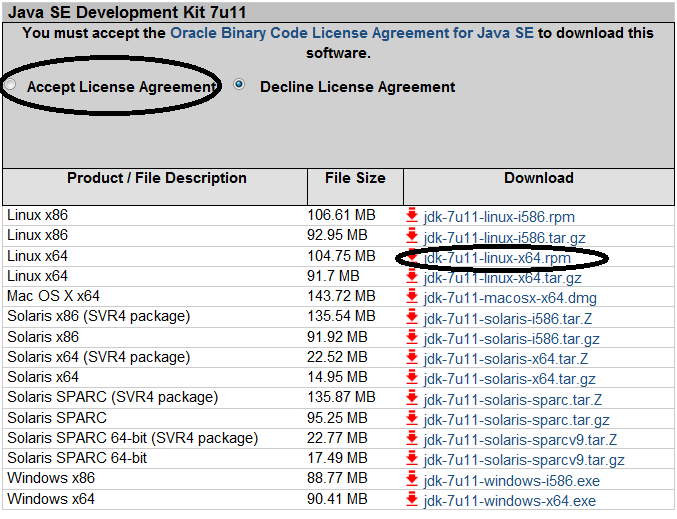
\includegraphics[width=.6\textwidth]{figs/5163os_02_04.png}
  \caption{Downloading Oracle JDK}\label{fig:oracle.jdk}
\end{figure} 
\subsection*{How to do it}
Use the following recipe to install Java and other tools:

Install Oracle Java with command (assuming we put the downloaded Java package to the home directory: \\
\verb|$ sudo yum localinstall ~/java-package-*.rpm|

Verify the installation with command: \\
\verb|$ java -version|

If Java is correctly installed, the output should be similar to the following:
\lstset{style=bashstyle}
\begin{lstlisting}
java version "1.6.0_33"
Java(TM) SE Runtime Environment (build 1.6.0_33-b04)
Java HotSpot(TM) 64-Bit Server VM (build 20.8-b03, mixed mode)
\end{lstlisting}

Use the following command to install necessary tools: \\
\verb|$ sudo yum -y install wget rsync nmap|

If these packages have been specified in the installation kickstart file, this step will be optional.

\subsection*{How it works}
wget\emph{\index{wget}} is a software tool for transferring files using HTTP, HTTPS and FTP protocols. It is none interactive and can be used from command line and scripts for file download. For more information please visit \href{http://www.gnu.org/software/wget/}{http://www.gnu.org/software/wget/}.

rsync\emph{\index{rsync}} is an open source tool that provides fast and incremental file transfers. It is widely used for file copying and synchronization under Linux. For more information about rsync, please visit \url{http://rsync.samba.org/}.

nmap\emph{\index{nmap}} stands for Network Mapper. It is a famous tool for network exploration and security auditing. We can use nmap to scan large networks and identify security problems. For example, to scan the service on local machine, we can use the following command:\\
\verb|$ nmap localhost|

And we can get output similar to the following:
\lstset{style=bashstyle}
\begin{lstlisting}
Starting Nmap 6.01 ( http://nmap.org ) at 2013-01-26 23:52 EST
Nmap scan report for localhost (127.0.0.1)
Host is up (0.0021s latency).
rDNS record for 127.0.0.1: localhost.localdomain
Not shown: 995 closed ports
PORT    STATE SERVICE
21/tcp  open  ftp
22/tcp  open  ssh
25/tcp  open  smtp
111/tcp open  rpcbind
631/tcp open  ipp

Nmap done: 1 IP address (1 host up) scanned in 0.14 seconds
\end{lstlisting}

The output tells us that the local machine has the following services running: \emph{ftp, ssh, smtp, rpcbind} (service for remote procedure calls) and \emph{jpp} (service for Java packaging).

Similarly, we can use the following command to scan IP segment 10.0.1.*: \\
\verb|$ nmap 10.0.0.*|

The command will give us service information of each host under the IP segment from 10.0.0.1 to 10.0.0.255.

\subsection*{There's more}
Under Linux, we can use the man command to get the usage of a command. For example, to get usage of wget, we can use {\emph \textbf man wget}.

If more detailed information about a command is desired, we can use the info command. For example, command info wget gives more details about command wget.

\section{Configuring SSH}
SSH\index{SSH} is the de facto standard protocol for secure data connection and remote command execution. Proper configuration of SSH is required for Hadoop installation. In this section, we are going to learn how to configure SSH on the cluster nodes. Specifically, we are discussing how to configure SSH for password-less login to a remote machine.

\subsection*{Getting ready}
Start up the SSHD service\index{SSHD service} on all the cluster nodes (both slave nodes and the master node) with command: \\
\verb|$ sudo service sshd start|

Make the service survive system reboot with command: \\
\verb|$ sudo chkconfig sshd on|

Verify that sshd works properly with command from master node: \\
\verb|$ ssh hduser@slave1|

If it is the first time to login to the host, we will get message similar to the following:
\lstset{style=bashstyle}
\begin{lstlisting}
The authenticity of host 'hdslave.host(10.0.0.1)' can't be established.
RSA key fingerprint is 7c:e0:61:3b:b6:70:07:ab:65:f9:bf:2d:90:77:1b:57.
Are you sure you want to continue connecting (yes/no)?
\end{lstlisting}

We need to type in yes and then provide the password for user hduser to login to the host.
\subsection*{How to do it...}
Use the following recipe to configure password-less login\index{password-less login}: \\
Login to the master node from the cluster administrator machine with the following command: \\
\verb|$ ssh hduser@master|

Use a text editor to modify the SSHD service configuration file \verb|/etc/ssh/ssh_config| by changing the following line: \\
\verb|#   StrictHostKeyChecking ask|

to: \\
\verb|StrictHostKeyChecking no|

Restart the SSHD server with command: \\
\verb|$ sudo service sshd restart|

Generate private and public keys with command: \\
\verb|$ ssh-keygen|

Press enter three times until this command finishes. A public key file \verb|~/.ssh/id_rsa.pub| and a private key file: \verb|~/.ssh/id_rsa| will be generated.

Copy the public key\index{public key} file to the remote machine with command: \\
\verb|$ ssh-copy-id slave1|

Test the configuration with command: \\
\verb|$ ssh hduser@slave1|

If we can login without entering the password, then the configuration is successful!
\subsection*{How it works}
When we run command \verb|ssh-copy-id hdslave.host|, we actually append the content of the public key file on local machine into file \verb|~/.ssh/authorized_keys| on the remote machine. Next time when we login, the public key string in file \verb|~/.ssh/authorized_keys| on the remote machine and local private key will be used for the login authentication process.
\subsection*{There's more...}
Configuration of password-less login failure can be caused by many reasons, for example, the configuration of firewall\index{firewall} (or iptables, to be more specific), SELinux and even the SSHD server itself. We will discuss methods to deal with these potential problems.
\subsubsection*{Erroneous SSH settings}
If the \verb|/etc/ssh_config| file contains the following lines:
\begin{verbatim}
RSAAuthentication no
PubkeyAuthentication no
\end{verbatim}

It means that the public key authorization\index{authorization} has been disabled. We need to change these two lines to the following:
\begin{verbatim}
RSAAuthentication yes
PubkeyAuthentication yes
\end{verbatim}

Make sure that the SSHD service has been successfully restarted on the remote machine with command: \\
\verb|$ sudo service sshd restart|

Manually check the \verb|~/.ssh/authorized_hosts| file on the remote host and see if the local machine's public key string has been appended. If not, we can manually append the local machine's public key to the \verb|~/.ssh/authorized_hosts| on the remote machine with commands:
\lstset{style=bashstyle}
\begin{lstlisting}[language=bash]
$ scp ~/.ssh/id_rsa.pub hduser@hdslave.host:~/
$ ssh hduser@hdslave.host -C "cat ~/id_rsa.pub >> ~/.ssh/authorized_hosts"
\end{lstlisting}

Log out of the remote machine and login again, if problem persists, go to the next step.
\subsubsection*{Erroneous iptables configuration}
Check the status of iptables with command: \\
\verb|$ sudo iptables -L|

If no rules are printed, go to the next step, otherwise, disable iptables\index{iptables} by flushing all the existing rules with command: \\
\verb|$ sudo iptables -F|

If problem persists, go to the next step.
\subsubsection*{Erroneous SELinux configuration}
Security Enhanced Linux (SELinux\index{SELinux}) is a Linux feature that provides the mechanism for supporting access control security policies. SELinux that is in enforcing mode can block the password-less login operation. We can check the current SELinux status with the following command: \\
\verb|$ getenforce|

If we get output similar to the following: \\
\commandoutput{Enforcing}

The output means SELinux is currently in enforcing mode, we need to put it in permissive mode with command: \\
\verb|$ sudo setenforce 0|

Alternatively, we can disable SELinux by editing file \verb|/etc/selinux/config| and change \verb|SELINUX=enforcing| to \verb|SELINUX=disabled|. Note that system reboot is required for the changes to take effect in this method.

\subsection*{See also}
\begin{itemize}
  \item Creating kickstart file and boot media
\end{itemize}
